\chapter{Stochastic Series Expansion}

	\section{Path integral}

		The path integral offers a way to deal with the Boltzmann operator $e^{-\beta \mc H}$ and especially its trace. This is useful when exact diagonalization becomes hard to be done. 

		Start with writing
		\be Z = \tr e^{-\beta \mc H} = \tr \prod_{l=1}^L e^{-\Delta_\tau \mc H} \ee
		with $\Delta_\tau = \frac{\beta}{L}$. A complete basis can be inserted between each branch, since the trace can be expressed as a sum of diagonal elements in any basis
		\be \begin{split} Z &= \sum_{\alpha_0} \cdots \sum_{\alpha_{L-1}} \mel{\alpha_0}{e^{-\Delta_\tau \mc H}}{\alpha_{L-1}} \cdots \mel{\alpha_1}{e^{-\Delta_\tau \mc H}}{\alpha_0} \\ &= \sum_{\{\alpha\})} W(\{\alpha\})) \end{split} \ee
		The argument in the exponential can be viewed as the Schrödinger time evolution operator $e^{-it\mc H}$ with the identification $\hbar=1$ and the imaginary time $t=-i\Delta_\tau$. The $W(\{\alpha\})$ are the weights of a world line configuration $\{\alpha\})$.

	\section{Series expansion representation}

		Before the path integral was introduced in this subject, the series expansion of the operator was predominant. Then a more general method, the stochastic series expansion, revived it to compute traces exactly by also sampling them.	Construct a configuration space for MC sampling by Taylor expanding the operator
		\be e^{-\beta \mc H} = \sum_{n=0}^\infty \frac{(-\beta)^n}{n!} \mc H^n \ee
		Introducing a complete basis
		\be Z = \sum_{n=0}^\infty \frac{(-\beta)^n}{n!} \sum_{\{\alpha\}_n} \mel{\alpha_0}{\mc H}{\alpha_{n-1}} \cdots \mel{\alpha_1}{\mc H}{\alpha_0} \label{eq:ZgenSSE} \ee
		Taking a boson system with only the kinetic energy, the Hamiltonian is 
		\be \mc H = - \sum_{\ev{ij}} (a^\dagger_i a_j + a^\dagger_ja_i) \ee
		and in this case, all the matrix element are the same so that
		\be W(\{\alpha\}_n) = \frac{\beta^n}{n!} \ee
		Also, the weights are positive definite, for bosons systems and quantum spins without frustration in the off-diagonal terms. Follow under this assumption.

		The energy is expressed as
		\be \begin{split} E &= -\pdv{\ln Z}{\beta} = \ev{\mc H} = \frac 1 Z \tr \mc H e^{-\beta \mc H} \\ &= \frac 1 Z \sum_{n=0}^\infty \frac{(-\beta)^n}{n!} \sum_{\{\alpha\}_{n+1}} \mel{\alpha_0}{\mc H}{\alpha_n} \cdots \mel{\alpha_1}{\mc H}{\alpha_0} \\ &= - \frac 1 Z \sum_{n=1}^\infty \frac{(-\beta)^n}{n!} \frac n \beta \sum_{\{\alpha\}_n} \mel{\alpha_0}{\mc H}{\alpha_n} \cdots \mel{\alpha_1}{\mc H}{\alpha_0} \\ &= - \frac 1 Z \sum_{n=0}^\infty \frac{(-\beta)^n}{n!} \frac n \beta \sum_{\{\alpha\}_n} \mel{\alpha_0}{\mc H}{\alpha_n} \cdots \mel{\alpha_1}{\mc H}{\alpha_0} \end{split} \label{eq:EmatchSSE} \ee
		and \eqref{eq:ZgenSSE} and \eqref{eq:EmatchSSE} match considering $\frac n \beta$ as the energy estimator. Thus
		\be E = -\frac{\ev n}{\beta} \ee
		If the Hamiltonian is written as
		\be \mc H = -\sum_i \mc H_i \ee
		then there is an expression for the expectation value of an individual $\mc H_i$ which is the average number of times it appears in the expansion of the partition function
		\be \ev{\mc H_i} = \frac{\ev{n_i}}{\beta} \ee
		Actually, one can take $n=\infty$ in the expression for the energy. But one can truncate it at $n_\text{max}\propto N\beta$ in practice. Take for instance the specific heat
		\be C = \pdv{E}{\beta} = \ev{n^2} - \ev{n}^2 - \ev n \ee
		When $T\to 0$, $C\to 0$ and then $\ev{n^2} - \ev{n}^2 \sim \ev n$. Hence, the variance of the distribution of $n$ goes like $\ev n$ and therefore the distribution vanishes exponentially beyond some $n_\text{max}$.

	\section{SSE for the $S=\frac12$ Heisenberg model}

		Consider the Heisenberg Hamiltonian as a sum of bond operators
		\be \mc H_b = J_b \vb* S_{i(b)} \cdot \vb* S_{j(b)} \ee
		with the lattice encoded as a list of sites $[i(b), j(b)]$ connected by the bond $b=1,\dotsc, N_b$. A positive definite SSE can be constructed for any bipartite lattice, for $i(b)$ in sublattice $A$ and $j(b)$ in $B$. Take $J_b=J>0$.

		One can further divide the Heisenberg interaction into its diagonal and off-diagonal parts in the $z$-component of the spin. Thus define bond operators
		\be \begin{split} \mc H_{1,b} &= \frac 1 4 - S^z_{i(b)} S^z_{j(b)} \\ \mc H_{2,b} = \frac 1 2 [ S^+_{i(b)} S^-_{j(b)} + S^-_{i(b)} S^+_{j(b)}] \end{split} \ee
		which implies the Hamiltonian
		\be \mc H = \frac{JN_b}{4} -J \sum_{b=1}^{N_b} [\mc H_{1,b} - \mc H_{2,b}] \label{eq:HheisenSSE} \ee
		The starting point of the SSE algorithm for this Hamiltonian is to write the partition function as
		\be Z = \sum_\alpha \sum_{n=0}^\infty (-1)^{n_2} \frac{\beta^n}{n!} \sum_{S_n} \ev{\prod_{p=0}^{n-1}\mc H_{a(p),b(p)}}{\alpha} \ee
		with $\beta=\frac J T$ having absorbed the coupling, $S_n$ the product of the bond operators
		\be S_n = [a(0),b(0)],[a(1),b(1)], \dotsc,[a(n-1),b(n-1)] \ee
		and $n_2$ is the number of off-diagonal operators. The action on the state
		\be \ket \alpha = \ket{S^z_1,\dotsc,S^Z_N} \ee
		by the string of operators, one gets a succession, propagated states
		\be \ket{\alpha(n)} \propto \prod_{p=0}^{n-1} \mc H_{a(p),b(p)} \ket \alpha \ee
		It is useful to observe that
		\be \begin{split} \mc H_{1,b} \ket{\uparrow_{i(b)} \uparrow_{j(b)}} = 0 &\qquad \mc H_{1,b} \ket{\downarrow_{i(b)} \downarrow_{j(b)}} = 0 \\ \mc H_{2,b} \ket{\uparrow_{i(b)} \uparrow_{j(b)}} = 0 &\qquad \mc H_{2,b} \ket{\downarrow_{i(b)} \downarrow_{j(b)}} = 0 \end{split} \ee
		and then the configurations $(\alpha,S_n)$ contributing to $Z$ must involve antiparallel spins, since
		\be \begin{split} \ev{\mc H_{1,b}}{\uparrow_{i(b)} \downarrow_{j(b)}} = \frac{1}{2} &\quad \mel{\downarrow_{i(b)} \uparrow_{j(b)}}{\mc H_{1,b}}{\uparrow_{i(b)} \downarrow_{j(b)}} = \frac 1 2 \\ \ev{\mc H_{2,b}}{\uparrow_{i(b)} \downarrow_{j(b)}} = \frac{1}{2} &\quad \mel{\uparrow_{i(b)} \downarrow_{j(b)}}{\mc H_{2,b}}{\downarrow_{i(b)} \uparrow_{j(b)}} = \frac 1 2  \end{split} \ee
		The propagation has to satisfy the periodicity condition
		\be \ket{\alpha(n)} = \ket{\alpha(0)} =\ket \alpha \label{eq:timeperiodicitycond} \ee
		for the partition function to be non-zero.

		It is practically useful to introduce a cut-off $L$, which should not cause any error. Define the unity operator as $\mc H_{0,0} = \mathbb 1$ and including $[a(p),b(p)] = [0,0]$ in the list, the partition function reads
		\be Z = \sum_\alpha \sum_{S_L} (-1)^{n_2} \frac{\beta^n (L-n)!}{L!} \ev{\prod_{p=0}^{L-1}\mc H_{a(p),b(p)}}{\alpha} \ee
		with $n$ the number of non-unity elements in the string in the fixed-length $S_L$. This formulation is useful since it fixes the number of operators to $n<L$ large enough, putting the remaining $L-n$ to unity, instead of changing the number $n$ of useful ones always. This explains the introduction of the $\binom{L}{n}$ since the unity operators can be put anywhere in the string. The weights become
		\be W(\alpha,S_L) = \left(\frac{\beta}{2}\right)^n \frac{(L-n)!}{L!} \ee

		\begin{figure}[h!]
            \centering
            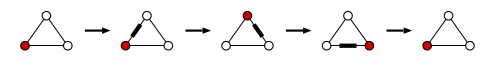
\includegraphics[scale=0.7]{graphs/threesitefrustSSE.png}
            \caption{Example of three off-diagonal operations bringing all spins back to their original states, each operator associated to a negative sign.}
            \label{fig:threesitefrustSSE}
        \end{figure}

		where the factor $\frac 1 2$ comes from all the non-zero amplitude and where $(-1)^{n_2}$ has been removed since they are taken to be always positive for a bipartite lattice. This is called the sign problem, which is not really a problem. Indeed, always an even number $n_2$ is required to satisfy the time periodicity condition \eqref{eq:timeperiodicitycond}. However, for frustrated systems such as the ones forming loops with an odd number of sites as in \autoref{fig:threesitefrustSSE}, the overall sign will be negative.

	\section{MC sampling}

		\begin{figure}[h!]
            \centering
            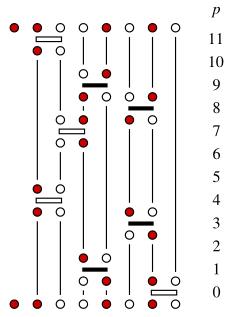
\includegraphics[scale=0.7]{graphs/linkedvertexSSE.png}
            \caption{Linked vertex storage configuration.}
            \label{fig:linkedvertexSSE}
        \end{figure}

		During the Monte Carlo sampling one will need to access operators and some properties of the propagated states also in non-sequential order—given an operator and the spins it acts on, one will need to to know which operators act on those spins next. It would be prohibitively time consuming to propagate a single state back and forth to extract this information, and also it would not be practical to store all the propagated states. Therefore use also another kind of data structure, in which the connectivity of the operators is explicit and represented as a network in a compact way. This linked vertex	structure is illustrated in \autoref{fig:linkedvertexSSE}. For the Heisenberg Hamiltonian considered, the vertices allowed are in \autoref{fig:verticesallowedSSE}. The goal here is to MC sample the partition function. 

		\begin{figure}[h!]
            \centering
            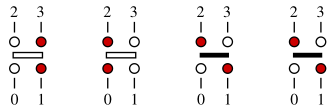
\includegraphics[scale=0.7]{graphs/verticesallowedSSE.png}
            \caption{Allowed vertices for the Heisenberg model considered.}
            \label{fig:verticesallowedSSE}
        \end{figure}

		The diagonal updates are the updates of single diagonal operators that can be carried out sequentially at locations $p=0,\dotsc, L-1$ in $S_L$. There is not constraint in the update $[1,b]_p \to [0,0]_p$ corresponding to the removal of a diagonal operator. The insertion of a diagonal operator $ [0,0]_p \to [1,b]_p$ is nonetheless constrained by the fact the the spins on bond $b$ must be antiparallel in the propagated state $\ket{\alpha(p)}$. The transition probabilities come from the expression for the weights. But one need to be careful that the selection probabilities depend on the choice of update. Writing
		\be P(A\to B) = P_\text{select}(B) P_\text{accept}(A \to B) \ee
		with the selections
		\be \begin{split} [1,b]_p \to [0,0]_p &\implies P_\text{select}([1,b]_p \to [0,0]_p) = 1 \\ [0,0]_p \to [1,b]_p &\implies P_\text{select}([0,0]_p \to [1,b]_p) = \frac{1}{N_b} \end{split} \ee
		since the diagonal operators can be put on the bond $b$ among all $N_b$ possible whereas there only one way to update to unity. Therefore
		\be \begin{split} P_\text{accept}([1,b]_p \to [0,0]_p) &= \min\left[ \frac{W(\alpha,S_L,n-1)}{W(\alpha,S_L,n)} \frac{1}{N_b},1 \right] \\ &= \min\left[\frac{2(L-n+1)}{\beta N_b},1 \right] \\ P_\text{accept}([0,0]_p \to [1,b]_p) &= \min\left[ \frac{W(\alpha,S_L,n+1)}{W(\alpha,S_L,n)} N_b,1 \right] \\ &= \min\left[\frac{\beta N_b}{2(L-n)},1 \right] \end{split} \ee
		where $n$ is the number of operators before the update. This satisfies the detailed balance condition, which can be checked quite easily.

		The off-diagonal updates have to involve at least two operators. In fact, involve an even number of them by periodicity conditions. For the Heisenberg model considered, use the loop updates that correspond to constructing a loop of generators connected by the links. For instance, an operator-loop is shown on \autoref{fig:SSEloop}. The goal is to flip the loop, that is flipping the spins along the loop as well as operators themselves. A loop cannot cross an operator since parallel spins acted upon by an operator are prohibited. To explore all phase space --- ergodicity --- one cannot just put and off-diagonal operator, then take the spins in a found loop and flip them with operators.

		\begin{figure}[h!]
            \centering
            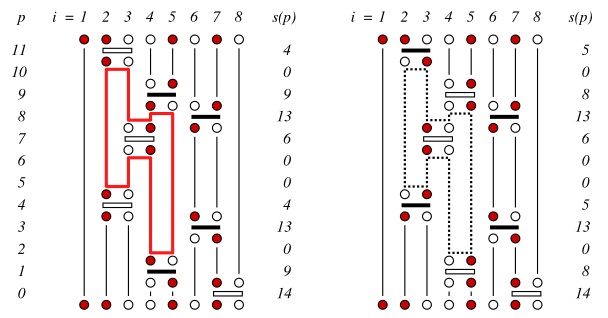
\includegraphics[scale=0.5]{graphs/SSEloop.png}
            \caption{SSE configuration with one loop shown before (left) and after (right) the operation of flipping spins and operators has been performed.}
            \label{fig:SSEloop}
        \end{figure}

		A MC step is then defined as
		\begin{itemize}
			\item Start with a randomly initialized spin state and initialize $S_L$ so that its elements are $[0,0]$ for all.
			\item By sequentially going through all elements of $S_L$, insert and remove diagonal operators according to the acceptance probabilities.
			\item After a full sequence of diagonal updates, construct and flip/accept a loop with a certain probability --- $\frac 1 2$ in the case of the Heisenberg model considered.
		\end{itemize}

	\section{Observables}

		In general, the thermal expectation value is
		\be \ev O = \frac 1 Z \tr Oe^{-\beta \mc H} \ee
		and since the trace is cyclic, one can put the $O$ anywhere. For $O$ diagonal $O\ket{\alpha(p)} = O_p \ket{\alpha(p)}$, the estimator of $O$ can be taken as 
		\be \ev{\bar O} = \frac 1 L \sum_{p=0}^{L-1} O_p \ee
		In practice, one can take the partial summation over every $N^\text{th}$ time slice for instance since states separated by a small number of slices are not very different in contrast to states separated by a large number of them. 

		Finally, the energy is such that
		\be E = -\frac{\ev n}{\beta} \ee
		and thus the more the non-trivial --- non-identity --- operators, the smaller the energy.


